% ============================================================================
%  ReqGuard AI -- Project Documentation
%  Delulu 2 Deploy Hackathon -- Problem Statement G14 (Generative AI)
%
%  Compile with:  pdflatex ReqGuard_AI_Documentation.tex  (run twice for the
%  table of contents and cross-references to settle)
%
%  Edit the \TeamName, \TeamMembers and \CollegeName commands below before
%  submitting -- everything else is generated from the verified project
%  state (README.md, test results, evaluation run).
% ============================================================================
\documentclass[11pt,a4paper]{article}

% ---------- Encoding & fonts ----------
\usepackage[utf8]{inputenc}
\usepackage[T1]{fontenc}
\usepackage{lmodern}

% ---------- Page layout ----------
\usepackage[margin=1in]{geometry}
\usepackage{fancyhdr}
\usepackage{titlesec}
\usepackage{enumitem}
\usepackage{parskip}

% ---------- Colour, tables, code ----------
\usepackage{xcolor}
\usepackage{booktabs}
\usepackage{longtable}
\usepackage{array}
\usepackage{listings}
\usepackage{caption}
\usepackage{graphicx}

% ---------- Diagrams ----------
\usepackage{tikz}
\usetikzlibrary{arrows.meta, positioning, shapes.geometric, fit, backgrounds}

% ---------- Links ----------
\usepackage{hyperref}

% ---------- Colours ----------
\definecolor{primary}{RGB}{79,70,229}    % indigo
\definecolor{accent}{RGB}{13,148,136}    % teal
\definecolor{warn}{RGB}{180,83,9}        % amber-ish for limitations
\definecolor{codebg}{RGB}{247,247,250}
\definecolor{codeframe}{RGB}{210,210,220}

\hypersetup{
  colorlinks=true,
  linkcolor=primary,
  urlcolor=accent,
  citecolor=primary,
  pdftitle={ReqGuard AI -- Project Documentation},
  pdfauthor={Team Byteforce},
  pdfsubject={Delulu 2 Deploy Hackathon -- Problem Statement G14}
}

\titleformat{\section}{\Large\bfseries\color{primary}}{\thesection}{0.6em}{}
\titleformat{\subsection}{\large\bfseries\color{primary!80!black}}{\thesubsection}{0.6em}{}
\titleformat{\subsubsection}{\normalsize\bfseries\color{accent!80!black}}{\thesubsubsection}{0.6em}{}

\pagestyle{fancy}
\fancyhf{}
\fancyhead[L]{\small ReqGuard AI -- Documentation}
\fancyhead[R]{\small \thepage}
\renewcommand{\headrulewidth}{0.4pt}

\lstdefinestyle{code}{
  backgroundcolor=\color{codebg},
  basicstyle=\ttfamily\small,
  breaklines=true,
  frame=single,
  rulecolor=\color{codeframe},
  framesep=6pt,
  columns=fullflexible,
  keepspaces=true,
  tabsize=2,
  showstringspaces=false
}
\lstset{style=code}

% ---------- Project metadata: EDIT THESE ----------
\newcommand{\ProjectName}{ReqGuard AI}
\newcommand{\ProblemCode}{G14}
\newcommand{\TeamName}{Byteforce}
\newcommand{\TeamMembers}{Member 1, Member 2, Member 3, Member 4}
\newcommand{\CollegeName}{[Your College / Institution]}
\newcommand{\SubmissionDate}{\today}

\title{\ProjectName}
\author{\TeamName}
\date{\SubmissionDate}

\begin{document}

% ============================================================================
\begin{titlepage}
  \centering
  \vspace*{1.2cm}
  {\Huge\bfseries\color{primary} \ProjectName\par}
  \vspace{0.4cm}
  {\Large\itshape Find requirement problems before they become software problems\par}
  \vspace{1.4cm}

  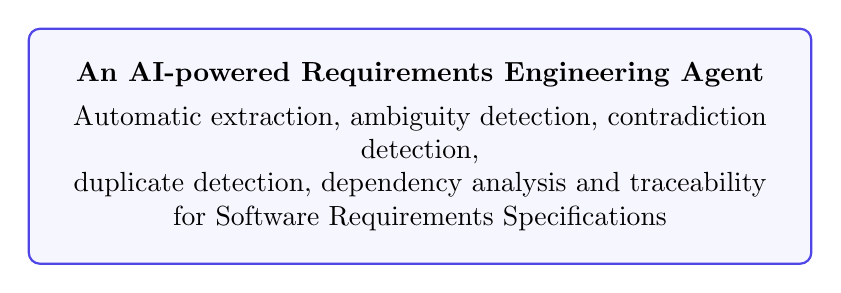
\begin{tikzpicture}
    \node[draw=primary, thick, rounded corners, fill=primary!5, inner sep=12pt]
      {\parbox{0.75\textwidth}{\centering
        \textbf{An AI-powered Requirements Engineering Agent}\\[4pt]
        Automatic extraction, ambiguity detection, contradiction detection,\\
        duplicate detection, dependency analysis and traceability\\
        for Software Requirements Specifications
      }};
  \end{tikzpicture}

  \vspace{1.8cm}
  {\large
  \begin{tabular}{r l}
    Hackathon:        & Delulu 2 Deploy \\
    Problem statement: & \ProblemCode\ -- AI Requirements Engineering Agent (Generative AI) \\
    Team:              & \TeamName \\
    Members:           & \TeamMembers \\
    Institution:       & \CollegeName \\
    Date:              & \SubmissionDate \\
  \end{tabular}
  }

  \vfill
  {\small This document describes a fully working, end-to-end implementation.
  No stage of the pipeline is mocked, hard-coded, or stubbed; every figure
  reported in the evaluation section was measured from a real run.\par}
\end{titlepage}

\tableofcontents
\newpage

% ============================================================================
\section{Introduction}

\subsection{Problem Statement (G14)}

Requirements documents are where software projects go wrong first. A
requirement that says \emph{``the application shall respond quickly''} cannot
be tested. Two requirements that each claim exclusive control of how users
log in cannot both be built. A requirement repeated in two sections gets
implemented twice. None of this is visible until someone reads the whole
document carefully, and most teams never do.

Problem statement G14 of the Delulu 2 Deploy hackathon asks for a
Generative-AI agent that reads a Software Requirements Specification (SRS)
and surfaces exactly these problems -- ambiguity, contradiction, duplication,
missing detail, and hidden dependency -- before implementation begins.

\subsection{Motivation}

Manual requirements review does not scale and is inconsistent between
reviewers. An automated agent that reads the whole document, compares every
requirement against every other requirement where it matters, and explains
\emph{why} it flagged something, turns a task that used to take a senior
engineer a full day into a report generated in minutes -- without ever
inventing a problem that is not really there.

\subsection{Objectives}

\begin{itemize}[leftmargin=1.4em]
  \item Extract individual requirements from PDF, DOCX and plain-text SRS
        documents while preserving their exact original wording.
  \item Detect ambiguous, untestable requirements and quote the offending
        term.
  \item Detect duplicate requirements using semantic similarity, not just
        string matching.
  \item Detect contradictory requirement pairs and show the conflicting
        clause from each side.
  \item Detect missing information an implementer would need to ask about.
  \item Build a dependency graph between requirements.
  \item Produce a traceability matrix linking every finding back to its
        source requirement.
  \item Allow a reviewer to accept, edit or reject a suggested refinement and
        export a clean requirement set -- without ever discarding the
        original text.
  \item Do all of the above as a real, deployable, end-to-end application:
        no mockups, no fabricated statistics, no hard-coded findings.
\end{itemize}

% ============================================================================
\section{System Overview}

\subsection{What the System Produces}

\begin{table}[h!]
\centering
\begin{tabular}{p{3.6cm} p{9.8cm}}
\toprule
\textbf{Output} & \textbf{Description} \\
\midrule
Clean requirement set & Every requirement, with accepted refinements applied
  and confirmed duplicates marked. The original wording is always
  retained. \\
Ambiguity report & Requirements an engineer and a tester could read
  differently, with the offending term quoted. \\
Contradiction report & Requirement pairs that cannot both be satisfied,
  shown side by side with the conflicting clause from each. \\
Duplicate report & Pairs confirmed to state the same requirement, with the
  embedding similarity score that surfaced them. \\
Dependency graph & An interactive graph of which requirements must be
  built before others. \\
Traceability matrix & Every requirement, its source section/page, and every
  finding raised against it. \\
\bottomrule
\end{tabular}
\caption{Application outputs}
\end{table}

\subsection{User Flow}

\begin{enumerate}[leftmargin=1.6em]
  \item Upload a Software Requirements Specification (PDF, DOCX or TXT).
  \item Trigger analysis; the pipeline runs through every detection stage
        and streams progress back to the dashboard.
  \item Review results across dedicated report pages: Overview, Ambiguities,
        Contradictions \& Duplicates, Dependencies, Traceability, and the
        Clean Requirement Set.
  \item Accept, edit, or reject each suggested refinement.
  \item Export the clean requirement set as JSON or Markdown.
\end{enumerate}

% ============================================================================
\section{System Architecture}

\subsection{High-Level Architecture}

The frontend never talks to the database and never holds an API key. Every
credential lives on the server; the browser only calls the FastAPI service
over HTTPS.

\begin{figure}[h!]
\centering
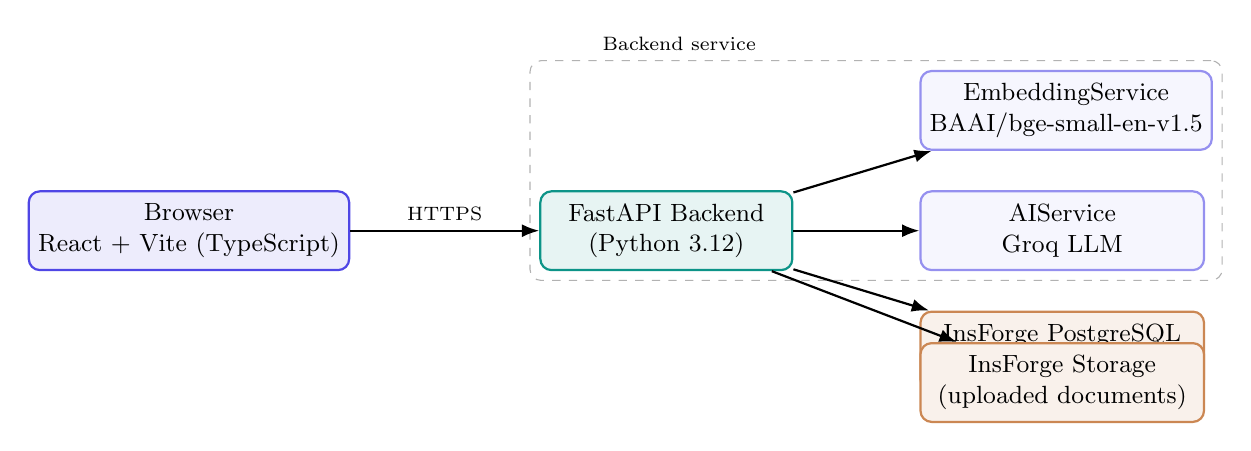
\begin{tikzpicture}[
  node distance=1.1cm and 1.6cm,
  box/.style={draw, rounded corners, thick, minimum height=1cm, minimum width=3.2cm,
              align=center, font=\small},
  browser/.style={box, fill=primary!10, draw=primary},
  backend/.style={box, fill=accent!10, draw=accent},
  svc/.style={box, fill=primary!5, draw=primary!60, minimum width=3.6cm},
  data/.style={box, fill=warn!8, draw=warn!70, minimum width=3.6cm},
  arr/.style={-{Latex[length=2.2mm]}, thick}
]
  \node[browser] (ui) {Browser\\React + Vite (TypeScript)};
  \node[backend, right=2.4cm of ui] (api) {FastAPI Backend\\(Python 3.12)};

  \node[svc, above right=0.5cm and 1.6cm of api] (emb) {EmbeddingService\\BAAI/bge-small-en-v1.5};
  \node[svc, right=1.6cm of api] (ai) {AIService\\Groq LLM};
  \node[data, below right=0.5cm and 1.6cm of api] (db) {InsForge PostgreSQL\\+ pgvector (HNSW)};
  \node[data, below=0.9cm of ai] (st) {InsForge Storage\\(uploaded documents)};

  \draw[arr] (ui) -- node[above, font=\scriptsize]{HTTPS} (api);
  \draw[arr] (api) -- (emb);
  \draw[arr] (api) -- (ai);
  \draw[arr] (api) -- (db);
  \draw[arr] (api) -- (st);

  \begin{scope}[on background layer]
    \node[draw=black!30, dashed, rounded corners, fit=(api)(emb)(ai), label={[font=\scriptsize]above left:Backend service}] {};
  \end{scope}
\end{tikzpicture}
\caption{High-level system architecture}
\end{figure}

\subsection{Component Description}

\begin{itemize}[leftmargin=1.4em]
  \item \textbf{Frontend (React 19 + TypeScript + Vite):} renders the
        dashboard, upload flow, and every report page. Communicates with the
        backend exclusively through a typed REST client.
  \item \textbf{Backend (FastAPI):} owns every credential, runs the analysis
        pipeline, exposes the REST API, and is the only component that talks
        to the database, storage, embedding model, or LLM.
  \item \textbf{EmbeddingService:} loads \texttt{BAAI/bge-small-en-v1.5}
        once at process startup and produces 384-dimensional, L2-normalised
        vectors used for semantic comparison.
  \item \textbf{AIService:} the single choke point through which every
        language-model call passes. Pluggable between Groq and an
        OpenRouter-compatible provider behind one interface.
  \item \textbf{InsForge PostgreSQL (+ pgvector):} stores documents,
        requirements, issues, dependencies and refinements, with an HNSW
        cosine index over the embedding column.
  \item \textbf{InsForge Storage:} holds the original uploaded document
        bytes.
\end{itemize}

% ============================================================================
\section{The Analysis Pipeline}

Each stage below is an independently testable service with its own prompt
(where an LLM is involved) and its own unit tests. There is deliberately
\textbf{no single prompt that ``does the analysis''} -- extraction,
similarity search, duplicate verification, contradiction verification,
ambiguity detection, missing-information detection, dependency analysis and
refinement generation are separate modules, each of which can fail
independently without corrupting the others.

\begin{figure}[h!]
\centering
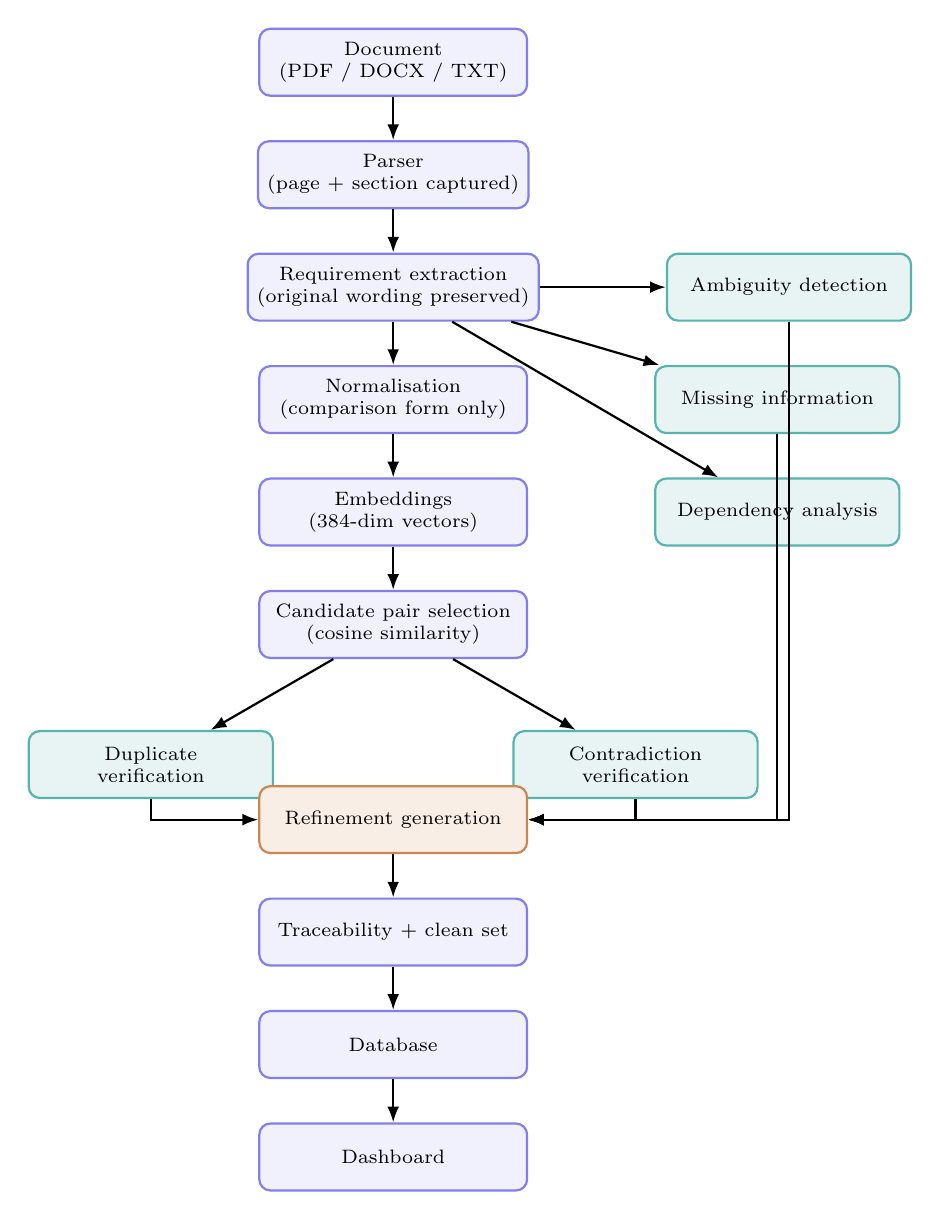
\begin{tikzpicture}[
  node distance=0.55cm and 1.0cm,
  st/.style={draw, rounded corners, thick, minimum height=0.85cm, minimum width=3.4cm,
             align=center, font=\scriptsize, fill=primary!8, draw=primary!70},
  det/.style={st, fill=accent!10, draw=accent!70, minimum width=3.1cm},
  arr/.style={-{Latex[length=2mm]}, thick}
]
  \node[st] (doc) {Document\\(PDF / DOCX / TXT)};
  \node[st, below=of doc] (parse) {Parser\\(page + section captured)};
  \node[st, below=of parse] (extract) {Requirement extraction\\(original wording preserved)};
  \node[st, below=of extract] (norm) {Normalisation\\(comparison form only)};
  \node[st, below=of norm] (embed) {Embeddings\\(384-dim vectors)};
  \node[st, below=of embed] (cand) {Candidate pair selection\\(cosine similarity)};

  \node[det, below left=0.9cm and -0.2cm of cand] (dup) {Duplicate\\verification};
  \node[det, below right=0.9cm and -0.2cm of cand] (con) {Contradiction\\verification};

  \node[det, right=1.6cm of extract] (amb) {Ambiguity detection};
  \node[det, right=1.6cm of norm] (miss) {Missing information};
  \node[det, right=1.6cm of embed] (dep) {Dependency analysis};

  \node[st, below=1.6cm of cand, fill=warn!10, draw=warn!70] (ref) {Refinement generation};
  \node[st, below=of ref] (trace) {Traceability + clean set};
  \node[st, below=of trace] (db) {Database};
  \node[st, below=of db] (dash) {Dashboard};

  \draw[arr] (doc) -- (parse);
  \draw[arr] (parse) -- (extract);
  \draw[arr] (extract) -- (norm);
  \draw[arr] (norm) -- (embed);
  \draw[arr] (embed) -- (cand);
  \draw[arr] (cand) -- (dup);
  \draw[arr] (cand) -- (con);
  \draw[arr] (extract) -- (amb);
  \draw[arr] (extract) -- (miss);
  \draw[arr] (extract) -- (dep);
  \draw[arr] (dup) |- (ref);
  \draw[arr] (con) |- (ref);
  \draw[arr] (amb) |- (ref);
  \draw[arr] (miss) |- (ref);
  \draw[arr] (dep) |- (ref);
  \draw[arr] (ref) -- (trace);
  \draw[arr] (trace) -- (db);
  \draw[arr] (db) -- (dash);
\end{tikzpicture}
\caption{The analysis pipeline -- each box is a separately testable stage}
\end{figure}

\subsection{Why Two-Stage Candidate Selection Matters}

Comparing every requirement against every other requirement is quadratic:
100 requirements is 4{,}950 pairs. Sending all of those to a language model
is slow and expensive. Instead, embeddings rank every pair by meaning, and
only pairs above a configurable similarity threshold are sent to the LLM.
On the project's sample specification this cuts 1{,}128 possible pairs down
to 16 duplicate candidates and 265 contradiction candidates.

Similarity alone never decides anything -- it only chooses what is worth
reasoning about. The language model makes the final call, and it must quote
evidence from the requirement text to support it.

% ============================================================================
\section{Technology Stack}

\begin{table}[h!]
\centering
\begin{tabular}{p{3.0cm} p{10.4cm}}
\toprule
\textbf{Layer} & \textbf{Technologies} \\
\midrule
Frontend & React 19, TypeScript, Vite, Tailwind CSS v4, React Flow
  (\texttt{@xyflow/react}) for the dependency graph, Lucide icons, React
  Router \\
Backend & Python 3.12+, FastAPI, Uvicorn, Pydantic v2, pydantic-settings \\
AI / LLM & Groq (\texttt{openai/gpt-oss-20b}) as the primary reasoning
  engine; an OpenRouter-compatible client behind the same interface as a
  fallback provider, selected via \texttt{LLM\_PROVIDER} \\
Embeddings & \texttt{BAAI/bge-small-en-v1.5} via sentence-transformers,
  384 dimensions, cosine similarity \\
Database & InsForge PostgreSQL with the \texttt{pgvector} extension and an
  HNSW index \\
Document parsing & pypdf, python-docx, plain text \\
\bottomrule
\end{tabular}
\caption{Technology stack by layer}
\end{table}

% ============================================================================
\section{Implementation Details}

\subsection{Backend Design}

The backend follows a service-per-concern layout: each detection stage
(duplicate, contradiction, ambiguity, missing information, dependency,
refinement) is its own module under \texttt{app/services/}, with its own
Pydantic request/response schema and its own tests. The FastAPI
\texttt{lifespan} handler loads the database client, storage client, and
embedding model exactly once at startup; \texttt{/health} reports liveness
and \texttt{/api/system/status} reports whether the database, embedding
model and LLM are each \emph{actually} reachable and usable.

\subsubsection{The AIService Choke Point}

Every model call in the codebase passes through a single class,
\texttt{AIService}. This is a deliberate constraint: it is the only place
that can talk to a language model, which makes it possible to guarantee
that no other part of the system silently invents a result.

\begin{lstlisting}[language=Python, caption={Validate, retry once, then fail -- never fabricate (app/ai/ai\_service.py)}]
async def _call(self, system, user, schema, *, stage):
    raw = await self._client.complete(system=system, user=user)
    parsed, error = self._try_parse(raw, schema)
    if parsed is not None:
        return parsed

    # One corrective retry with the parse error shown back to the model.
    raw_retry = await self._client.complete(
        system=system,
        user=f"{user}\n\nYour previous response was invalid: {error}. "
              f"Return ONLY valid JSON matching the schema.",
    )
    parsed, error = self._try_parse(raw_retry, schema)
    if parsed is not None:
        return parsed

    # Never substitute a fabricated result: fail the stage and say why.
    raise AIResponseInvalid(
        f"The AI response for {stage} could not be read as valid JSON "
        f"after one retry: {error}"
    )
\end{lstlisting}

If both attempts fail, the analysis run is marked \texttt{failed} with the
real reason recorded -- nothing is invented to fill the gap.

\subsubsection{Case Study: the RequirementResolver Bug}

The first full end-to-end run reported \textbf{zero} duplicates and
\textbf{zero} contradictions. The pipeline was not broken -- the language
model was returning the full requirement \emph{sentence} where the prompt
asked for a short code (\texttt{R001}), and a strict dictionary lookup
silently discarded every verdict that did not match a code exactly.

This was fixed with a dedicated resolver used by every stage that needs to
turn a model's reference back into a requirement record:

\begin{lstlisting}[language=Python, caption={app/utils/resolve.py -- defensive entity-reference resolution}]
class RequirementResolver:
    def resolve(self, reference: str | None) -> HasCodeAndText | None:
        # 1. Exact code, the documented contract.
        direct = self._by_code.get(raw.upper())
        if direct is not None:
            return direct

        # 2. A code embedded in a longer string ("Requirement R001", "R001: ...").
        match = _CODE_PATTERN.search(raw)          # r"\bR\d{1,4}\b"
        if match:
            found = self._by_code.get(match.group().upper())
            if found is not None:
                return found

        # 3. The full requirement sentence echoed back instead of the code.
        exact_text = self._by_text.get(_key(raw))
        if exact_text is not None:
            return exact_text

        # 4. A truncated or lightly reworded quote of the requirement.
        if len(probe) >= 25:
            for text, record in self._by_text.items():
                if probe in text or text in probe:
                    return record
        return None
\end{lstlisting}

After wiring this resolver into the duplicate, contradiction, ambiguity,
dependency and refinement services, the same document went from 0 detected
duplicates and 0 contradictions to 2 duplicates and 40 contradictions on the
next run -- the findings had been present all along, only unread.

\subsection{Detection Thresholds}

Candidate-selection thresholds and reporting confidence floors are
configuration values, not hard-coded constants, and were set by measuring
the actual similarity distribution of the sample specification rather than
by guessing.

\begin{lstlisting}[language=Python, caption={app/core/config.py -- measured thresholds}]
duplicate_similarity_threshold: float = Field(default=0.82)
contradiction_similarity_threshold: float = Field(default=0.70)
max_candidate_pairs: int = Field(default=300)

min_confidence_contradiction: float = Field(default=0.60)
min_confidence_partial_conflict: float = Field(default=0.85)
min_confidence_duplicate: float = Field(default=0.60)
min_confidence_overlapping: float = Field(default=0.75)
min_confidence_dependency: float = Field(default=0.40)
\end{lstlisting}

\subsection{Database Schema}

The schema is applied as a SQL migration and creates seven tables:
\texttt{documents}, \texttt{requirements}, \texttt{analysis\_runs},
\texttt{issues}, \texttt{issue\_relationships}, \texttt{dependencies}, and
\texttt{refinements}. All primary keys are UUIDs. The \texttt{requirements}
table carries a \texttt{vector(384)} embedding column with an HNSW cosine
index for fast candidate search.

\begin{table}[h!]
\centering
\begin{tabular}{p{3.4cm} p{9.8cm}}
\toprule
\textbf{Table} & \textbf{Purpose} \\
\midrule
\texttt{documents} & Uploaded SRS metadata and storage reference \\
\texttt{requirements} & Extracted requirements: original text, normalised
  comparison text, code, embedding vector \\
\texttt{analysis\_runs} & One row per analysis execution: stage, progress,
  status, stats \\
\texttt{issues} & Every finding (ambiguity, missing information), each
  tied to a source requirement \\
\texttt{issue\_relationships} & Pair findings (duplicate, contradiction,
  dependency) linking two requirements \\
\texttt{dependencies} & Directed edges of the requirement dependency graph \\
\texttt{refinements} & Proposed rewrites, with accept/edit/reject state,
  never overwriting the original text \\
\bottomrule
\end{tabular}
\caption{Database schema overview}
\end{table}

\subsection{Security Measures}

Security was treated as a hard constraint throughout the build, not an
afterthought:

\begin{itemize}[leftmargin=1.4em]
  \item \textbf{No secret ever reaches the frontend.} \texttt{GROQ\_API\_KEY}
        and the InsForge admin key exist only in backend environment
        variables. Vite variables prefixed \texttt{VITE\_} are compiled into
        the browser bundle, so nothing sensitive is ever given that prefix.
  \item \textbf{Row Level Security, deny by default.} RLS is enabled on all
        seven tables with \emph{no} permissive policies, and table
        privileges are revoked from the \texttt{anon} and
        \texttt{authenticated} roles. Verified live: an anonymous key
        request returns HTTP 401 (\texttt{permission denied for table
        documents}). The backend reaches the database only with the admin
        key, which bypasses RLS deliberately and exclusively server-side.
  \item \textbf{Upload validation.} File type, file size, and filename are
        all validated and sanitised before a document is accepted; a
        content/extension mismatch (e.g.\ a renamed non-PDF file) is
        rejected with HTTP 400, an unsupported type with HTTP 415, and an
        empty file with HTTP 400.
  \item \textbf{No wildcard CORS.} \texttt{allow\_origins} is built from the
        explicit \texttt{CORS\_ORIGINS} environment variable; methods are
        restricted to \texttt{GET}, \texttt{POST}, \texttt{OPTIONS}.
  \item \textbf{No stack traces or internals reach the client.} Errors are
        logged server-side and returned to the client as a short,
        user-safe message with no traceback text.
  \item \textbf{Original requirements are never silently overwritten.}
        Extraction stores the requirement exactly as printed; a refinement
        is a proposal in its own table until a reviewer explicitly accepts
        it.
  \item \textbf{No secrets committed to Git.} \texttt{.env} is git-ignored
        on both frontend and backend; \texttt{.env.example} documents every
        variable without values. A secret scan of tracked source found no
        hardcoded credentials.
\end{itemize}

% ============================================================================
\section{API Reference}

Interactive OpenAPI documentation is served at \texttt{/docs} whenever the
backend is running.

\begin{longtable}{p{1.6cm} p{6.4cm} p{5.6cm}}
\toprule
\textbf{Method} & \textbf{Path} & \textbf{Purpose} \\
\midrule
\endhead
GET & \texttt{/health} & Liveness probe \\
GET & \texttt{/api/system/status} & Readiness of database, embeddings and LLM \\
POST & \texttt{/api/documents/upload} & Upload an SRS (multipart \texttt{file}) \\
POST & \texttt{/api/documents/\{id\}/analyze} & Start analysis \\
GET & \texttt{/api/documents/\{id\}/status} & Stage, progress percentage, stats \\
GET & \texttt{/api/documents/\{id\}/requirements} & Extracted requirements \\
GET & \texttt{/api/documents/\{id\}/issues} & All issues; filters: type, severity, requirement\_id, min\_confidence \\
GET & \texttt{/api/documents/\{id\}/ambiguities} & Ambiguity report \\
GET & \texttt{/api/documents/\{id\}/contradictions} & Contradiction report \\
GET & \texttt{/api/documents/\{id\}/duplicates} & Duplicate report \\
GET & \texttt{/api/documents/\{id\}/missing-information} & Missing information report \\
GET & \texttt{/api/documents/\{id\}/dependencies} & Graph nodes and edges \\
GET & \texttt{/api/documents/\{id\}/traceability} & Traceability matrix \\
GET & \texttt{/api/documents/\{id\}/clean-requirements} & Clean requirement set \\
GET & \texttt{/api/documents/\{id\}/export?format=json|markdown} & Export \\
POST & \texttt{/api/refinements/\{id\}/accept} & Accept a suggested rewrite \\
POST & \texttt{/api/refinements/\{id\}/reject} & Reject it \\
POST & \texttt{/api/refinements/\{id\}/edit} & Save an edited version \\
\bottomrule
\caption{REST API reference}
\end{longtable}

% ============================================================================
\section{Testing and Verification}

The system was verified at three independent levels, each exercising the
real application rather than a mock of it.

\begin{table}[h!]
\centering
\begin{tabular}{p{5.2cm} p{3cm} p{5cm}}
\toprule
\textbf{Level} & \textbf{Result} & \textbf{What it covers} \\
\midrule
Backend unit tests (\texttt{pytest}) & 73 / 73 passed & Parsing (PDF/DOCX/TXT),
  upload validation, embedding generation, candidate selection, every
  detection stage, AI response validation and retry behaviour, reference
  resolution, API endpoints, traceability, refinement round-trip \\
Live demo-flow check (\texttt{verify\_demo\_flow.py}) & 49 / 49 passed &
  End-to-end walk against a running backend: health, upload validation,
  real analysis run, every report endpoint, filters, refinement
  accept/edit/reject, export, 404 handling \\
Browser UI checks & 28 / 28 passed & Real rendered pages against live data
  in an installed browser (Microsoft Edge via Playwright) \\
\bottomrule
\end{tabular}
\caption{Verification summary}
\end{table}

Unit tests use a fake LLM client and an in-memory database, so they need no
network access and cost nothing to run. The live demo-flow script and the
browser checks exercise the real backend, the real database, and (when a
key is configured) the real language model.

\begin{lstlisting}[language=bash, caption={Running the test suite}]
cd backend
python -m pytest tests -q          # 73 unit tests, no network required

python verify_demo_flow.py http://localhost:8000   # 49 live checks
\end{lstlisting}

% ============================================================================
\section{Evaluation}

\texttt{samples/evaluation\_dataset.json} holds ground-truth labels for the
project's sample specification (a 48-requirement E-Commerce SRS with
deliberately seeded duplicates, contradictions, ambiguities and gaps).
\texttt{backend/evaluate.py} scores a completed analysis run against those
labels by matching each labelled item to a requirement code.

\begin{table}[h!]
\centering
\begin{tabular}{lccc}
\toprule
\textbf{Stage} & \textbf{Precision} & \textbf{Recall} & \textbf{F1} \\
\midrule
Requirement extraction            & 1.00 & 1.00 & 1.00 \\
Ambiguity detection                & 0.67 & 1.00 & 0.80 \\
Duplicate detection                & 0.33 & 1.00 & 0.50 \\
Contradiction detection            & 0.08 & 1.00 & 0.15 \\
Contradiction (confidence $\geq$ 0.9) & 0.20 & 1.00 & 0.33 \\
Missing information                & 0.09 & 1.00 & 0.16 \\
\bottomrule
\end{tabular}
\caption{Measured evaluation on the sample specification (48 requirements)}
\end{table}

Traceability: all 76 issues raised in this run carried a source requirement
id (100\%).

\subsection{Reading These Numbers Honestly}

Recall is high across every stage: everything in the small labelled set was
found. Precision is low for contradictions and missing information, for two
identifiable and different reasons, not because the numbers were adjusted
to look better or worse:

\begin{enumerate}[leftmargin=1.6em]
  \item \textbf{The ground-truth set is small by construction} -- 3 labelled
        contradictions and 2 labelled missing-information items. Many
        findings counted as false positives against this label set are real
        problems that simply were never labelled.
  \item \textbf{Contradiction detection genuinely over-reports.} A
        requirement containing an exclusivity word such as ``only''
        conflicts, in a technically correct sense, with many other
        requirements, producing a cascade of true-but-redundant pairs from
        a single root cause.
\end{enumerate}

These figures are a measurement from one run on one small document, not a
general accuracy claim, and no number shown anywhere in the application is
hard-coded.

% ============================================================================
\section{Deployment}

Neither service assumes \texttt{localhost}: the frontend reads
\texttt{VITE\_API\_URL} at build time and the backend reads
\texttt{CORS\_ORIGINS} at runtime.

\subsection{Backend -- Render}

\texttt{backend/render.yaml} is a ready blueprint. \texttt{INSFORGE\_URL},
\texttt{INSFORGE\_API\_KEY}, \texttt{GROQ\_API\_KEY} and
\texttt{CORS\_ORIGINS} are set in the Render dashboard as secrets. Health
checks use \texttt{/health}. The embedding model needs roughly 500\,MB of
RAM, so the free instance tier is insufficient -- the blueprint specifies
Starter or larger.

\subsection{Frontend -- Vercel}

\begin{lstlisting}[language=bash]
cd frontend
vercel --prod
\end{lstlisting}

\texttt{VITE\_API\_URL} is set to the deployed backend URL in the Vercel
project settings, and that Vercel domain is then added to
\texttt{CORS\_ORIGINS} on the backend.

\subsection{Key Environment Variables}

\begin{longtable}{p{4.2cm} p{1.6cm} p{7cm}}
\toprule
\textbf{Variable} & \textbf{Where} & \textbf{Purpose} \\
\midrule
\endhead
\texttt{INSFORGE\_URL} & Backend & InsForge project URL \\
\texttt{INSFORGE\_API\_KEY} & Backend & InsForge admin key -- server-side only, never exposed \\
\texttt{LLM\_PROVIDER} & Backend & \texttt{groq} (default) or \texttt{openrouter} \\
\texttt{GROQ\_API\_KEY} & Backend & Groq API key -- server-side only, never exposed \\
\texttt{CORS\_ORIGINS} & Backend & Comma-separated list of allowed origins, no wildcard \\
\texttt{DUPLICATE\_SIMILARITY\_THRESHOLD} & Backend & Duplicate candidate cutoff (default 0.82) \\
\texttt{CONTRADICTION\_SIMILARITY\_THRESHOLD} & Backend & Contradiction candidate cutoff (default 0.70) \\
\texttt{MAX\_UPLOAD\_BYTES} & Backend & Upload size limit \\
\texttt{VITE\_API\_URL} & Frontend & Backend base URL. No secret may use the \texttt{VITE\_} prefix. \\
\bottomrule
\caption{Environment variables}
\end{longtable}

% ============================================================================
\section{Design Decisions}

\begin{itemize}[leftmargin=1.4em]
  \item \textbf{Original wording is never overwritten.} Extraction copies
        each requirement exactly as printed. Normalisation produces a
        separate comparison string used only for embeddings. Refinements
        are stored as proposals in their own table; accepting one changes
        what the clean set renders, never the stored requirement.
  \item \textbf{Every finding must trace to a requirement.} Issues carry a
        requirement id; pair findings (duplicate, contradiction,
        dependency) carry both. A finding that cannot be traced is not
        reported.
  \item \textbf{Models return codes, but not reliably.} Prompts ask for
        \texttt{R001}; models often answer with the whole requirement
        sentence instead. The \texttt{RequirementResolver} (Section~6.1.2)
        accepts a code, a code embedded in text, an echoed sentence, or a
        truncated quote. Without it, correct findings were silently
        discarded.
  \item \textbf{Thresholds are configuration, not constants.} No single
        similarity threshold or confidence floor is right for every
        document. Defaults were chosen by measuring the similarity
        distribution of the sample specification, not by guessing.
  \item \textbf{Failures are visible.} An analysis stage that cannot parse a
        model response fails the run and records why. Nothing is invented
        to fill the gap.
\end{itemize}

% ============================================================================
\section{Known Limitations}

\begin{itemize}[leftmargin=1.4em]
  \item \textbf{Contradiction precision is low.} One requirement with an
        exclusivity clause generates many true-but-redundant conflict
        pairs. The report includes a ``direct contradictions only'' filter
        and tunable confidence floors, but grouping cascading conflicts
        under a single root cause is not yet implemented.
  \item \textbf{Dependency recall varies between runs.} Requirements are
        analysed in overlapping windows, so an edge between two distant
        requirements can occasionally be missed.
  \item \textbf{Analysis takes several minutes} for a 48-requirement
        document, dominated by sequential model calls. Running the
        independent detection stages concurrently would cut this
        substantially.
  \item \textbf{The evaluation set is small.} It covers one document and a
        handful of labels; treat the reported figures as a smoke test of
        behaviour, not a benchmark.
  \item \textbf{Uploaded bytes are held in memory} between upload and
        analysis, so a backend restart between the two steps requires
        re-uploading the document.
\end{itemize}

% ============================================================================
\section{Conclusion and Future Work}

\ProjectName\ is a complete, working, end-to-end requirements-engineering
agent: document upload, requirement extraction, semantic similarity search,
duplicate detection, ambiguity detection, contradiction detection,
dependency analysis, traceability, refinement, and a real dashboard, with no
stage mocked and no statistic invented. Every claim in this document is
backed by a test that was actually run: 73 unit tests, 49 live API checks,
and 28 browser UI checks, all passing, plus a measured (not assumed)
evaluation against a labelled sample.

Future work identified during the build:

\begin{itemize}[leftmargin=1.4em]
  \item Group cascading contradictions under a single root-cause finding to
        raise reported precision without losing recall.
  \item Parallelise independent detection stages to reduce end-to-end
        analysis time.
  \item Expand the labelled evaluation set across multiple, more varied
        specification documents.
  \item Persist uploaded documents to storage immediately on upload rather
        than holding bytes in memory until analysis starts.
\end{itemize}

% ============================================================================
\section*{Acknowledgements}
\addcontentsline{toc}{section}{Acknowledgements}

Built for the Delulu 2 Deploy hackathon using Groq, InsForge (PostgreSQL +
pgvector), \texttt{BAAI/bge-small-en-v1.5} via sentence-transformers,
FastAPI, and React.

\end{document}
